\newpage
\section{Architecture}
\label{Arc}



The architecture of the UAV based SDN system for wireless sensor networks.

\begin{figure}[htbp]
	\centering
	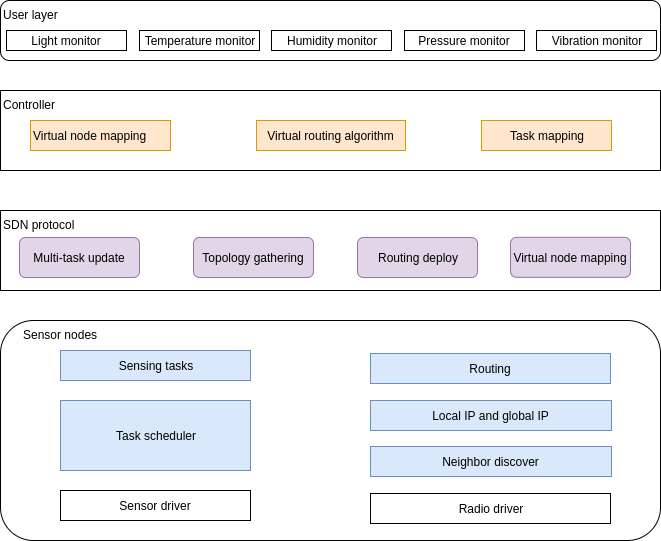
\includegraphics[width=3.5in]{./Figure/Architecture}
	\caption{Architecture of the system.}
	\label{Architecture}
\end{figure}




\begin{table*}[htbp]
	\caption{System API}
	\label{API}
	\centering
	\scalebox{0.9}{
	\begin{tabular}{|l|l|}
		\hline
		\makecell[tc]{\textbf{Structure \&\& Function}} & \makecell[tc]{\textbf{Description}} \\
		\hline
		\multicolumn{2}{|c|}{\textbf{Sensor Control Interface}}\\
		\hline
		struct node & Sensor node structure\\
		\hline
		struct nodeset & A set of sensor nodes \\
		\hline
		struct neighbor\_list & Neighbor infomation \\
		\hline
		struct energy\_item & Energy statistic information \\
		\hline
		struct flow\_table & Flow table \\
		\hline
		struct duty\_cycle\_table & Duty cycle control table \\
		\hline
		struct sensor\_enable\_table & All the nodes's states. Node state: \{on,off\} \\
		\hline
		switch\_node(node,state) & Turn on or turn off the node \\
		\hline
		get\_node\_info(node) & Get node's information, including  node's position, duty cycle, power, etc.\\
		\hline
		set\_node\_attr(node,attrTag,value) & Set node attribute, including  duty cycle, radio strength, etc. \\
		\hline
		get\_neighborlist(node) & Get the neighbor list of a node \\
		\hline
		\multicolumn{2}{|c|}{\textbf{UAV Application Interface}}\\
		\hline
		\multicolumn{2}{|c|}{\textbf{Routing}}\\
		\hline
		get\_topology() & Get the topology of the network\\
		\hline
		get\_flow\_table(node) & Get the flow table of a node \\
		\hline
		set\_flow(flow,node) & Set the flow of a node \\
		\hline
		\multicolumn{2}{|c|}{\textbf{AI Node selection}}\\
		\hline
		nodeset simple\_selection(nodeset) & Select sensor set by location information\\
		\hline
		nodeset SRSSS\_selection(dataset) & Select sensor set by AI algorithm based on sensing data\\
		\hline
		\multicolumn{2}{|c|}{\textbf{AI Energy Prediction}}\\
		\hline
		model\_selsct(modeltype) & Select an AI model\\
		\hline
		model.train(dataset,ratio) & Train an AI model with learning ratio on the data set\\
		\hline
		model.test(dataset) & Test the AI model on the data set\\
		\hline
		model.predict(node) & Do the energy prediction for a node \\
		\hline
		\multicolumn{2}{|c|}{\textbf{Multi-tasks}}\\
		\hline
		create\_scheduler() & Create a task scheduler \\
		\hline
		scheduler.create\_buffer() & Create a task buffer \\
		\hline
		scheduler.task\_buffer\_add(task,nodeset) & Add a new task to task buffer \\
		\hline
		scheduler.task\_buffer\_remove(task) & Remove a new task to task buffer \\
		\hline
		scheduler.task\_buffer\_update(task,nodeset) & Update a task to task buffer with a new nodeset \\
		\hline
		scheduler.task\_update() & Schedule the added or removed tasks in the buffer\\
		\hline
		\multicolumn{2}{|c|}{\textbf{Diagnosis}}\\
		\hline
		detect() & Detect problematic region with probes \\
		\hline
		get\_topical\_topology(nodeset) & Construct topical topology\\
		\hline
		diagnose\_network(topology,nodeset) & Diagnose the failure nodes or lossy links\\
		\hline
	\end{tabular}
	}
\end{table*}

\begin{lstlisting}[
	language={[ANSI]C},
	label=topology-update,caption={An example of deploy routing algorithm},
	keywordstyle=\color{blue!70},
	showstringspaces=false,
	commentstyle=\color{red!50!green!80!blue!70},
	frame=single,captionpos=t,
	rulesepcolor=\color{red!20!green!20!blue!20},
	basicstyle=\ttfamily]
topology = get_topology();
//calculate flowtable for each node
//based on topology
for(node in nodeset){
   node.flowtable =
      calculate_flowtable(topology);
}
//set flowtable for each node
for(node in nodeset){
   UAV fly to node;
   for(flow in node.flowtable)
        set_route(flow);
}

\end{lstlisting}

\begin{lstlisting}[language={[ANSI]C},label=AI,
	caption={An example of AI selection and Muti-tasks},
	keywordstyle=\color{blue!70},
	showstringspaces=false,
	commentstyle=\color{red!50!green!80!blue!70},
	frame=single,captionpos=t,
	rulesepcolor=\color{red!20!green!20!blue!20},
	basicstyle=\ttfamily]
AI_Multitasks(taskset){
   create_scheduler();
   scheduler.create_buffer();

   for(task in taskset)
      scheduler.task_buffer_add(
         task,
         defaultset);

   scheduler.task_update();
   ...
   ...
   for(task in scheduler.task_buffer){
      data = get_collected_data();
      nodeset =
         SRSSS_selection(dataset);
      scheduler.task_buffer_update(
         task,
         nodeset);
   }
   scheduler.task_update();
}

\end{lstlisting}

